%!TEX root = ../physical-olympics-2.tex
\chapter{相与相变摘要}


\section{相平衡}

\begin{itemize}
	\item 相平衡条件:\,等温等压,\,化学势相等:\,
	\[\mu_1(T,\,p)=\mu_2(T,\,p)\]

	即三种平衡同时被满足:\,热学,\,力学与化学平衡.

	\item 若$\mu_1>\mu_2$,\,粒子从势高的向势低的自发相变.\,如某温度下未饱和的水蒸气内化学势就会低于水中的化学势.

	\item 除了这三个量相等,\,摩尔熵$s$,\,摩尔体积$v$,\,数密度$n$两相平衡时都可以不相等.

	\item \emph{相变潜热}(latent heat)指等温等压条件下的吸热,\,所以是摩尔焓的增量:
	\[Q=\nu l=h_2-h_1=u_2-u_1+p(v_2-v_1)\]

	\item $0\cdgr$下若把水的比热容记做$1{\rm cal/g\cdot K}$,\,那么水的溶解热与汽化热为$80{\rm cal/g}$与$600{\rm cal/g}$,\,$100\cdgr$下汽化热降低到只有$540{\rm cal/g}$.\,冰和水蒸气的比热容几乎刚好只有水的一半$0.5{\rm cal/g\cdot K}$
\end{itemize}

\section{气液相变}
\begin{wrapfigure}[9]{o}[-10pt]{7cm}
\centering
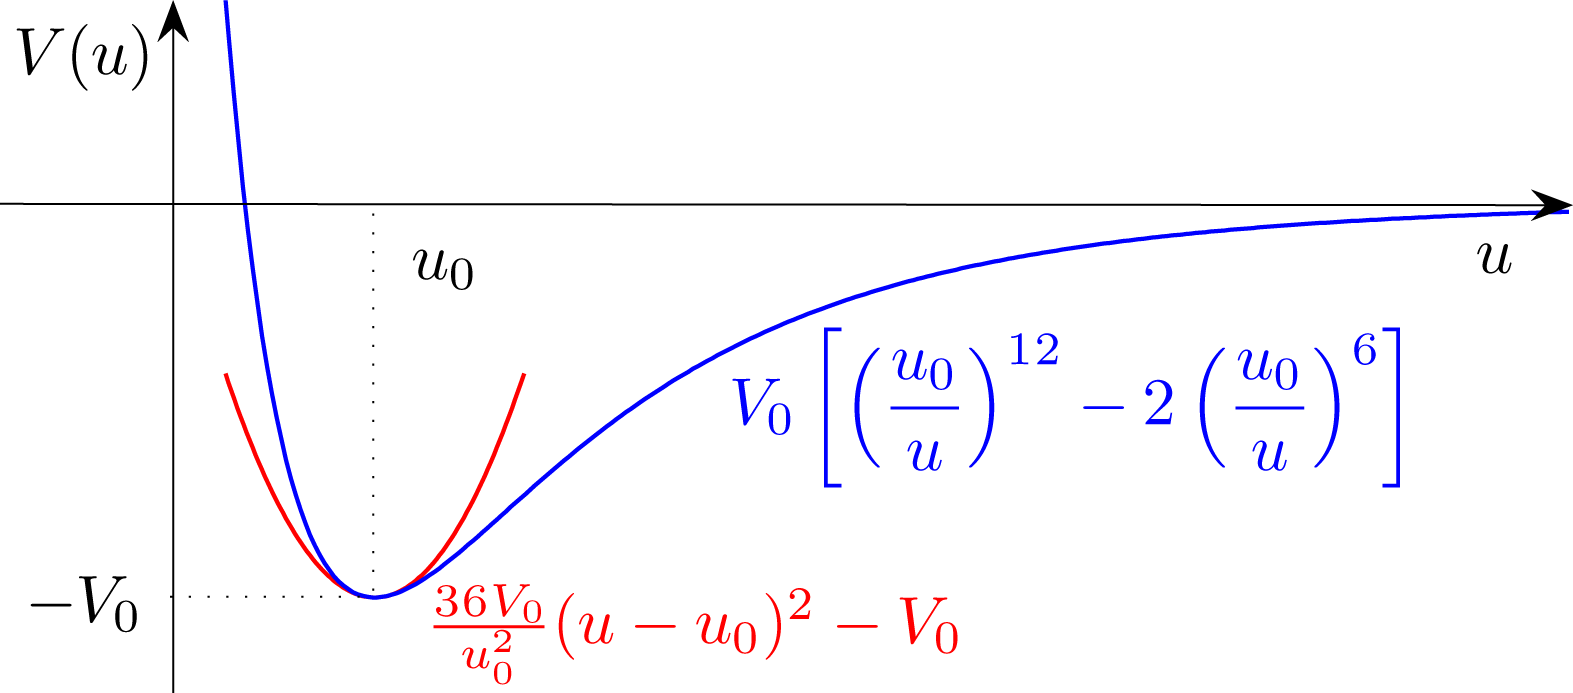
\includegraphics[width=7cm]{image/5-3-6.png}
\caption{范氏等温线}
\end{wrapfigure}
首先\emph{范德瓦尔斯方程}(van der Waals equation):
\[p=\frac{\nu RT}{V-\nu b}-\frac{\nu^2 a}{V^2}\]
\begin{itemize}
	\item 用范德瓦尔斯方程同时可以描述气体和液体,\,低于临界温度$T_c=8a/27Rb$时$p-V$曲线不再单调.\,提供了等温等压等化学势相平衡的可能性.\,事实上在\emph{麦克斯韦等面积法则}(Maxwell's equal area rule)决定的两点处能够相平衡.\,这定义了气液两相的分歧背后的数学原因.
	\item 汽化的熵变其实简单地决定了潜热:
	\[l=T(s_{\rm g}-s_{\rm l})\]
	\end{itemize}

	\begin{itemize}
	\item 两相共存时压强与温度的导数关系,\,也就是\emph{克劳修斯-克拉伯龙关系}(Clausius-Clapeyron relation):
	\[\frac{\ud p}{\ud T}=\frac{s_{\rm g}-s_{\rm l}}{v_{\rm g}-v_{\rm l}}=\frac{l}{T(v_{\rm g}-v_{\rm l})}\]
	
	\item \emph{蒸发}(evaporation):\,由于大气的存在,\,水蒸气在空气中仅是分压,\,不等于水的压强,\,但是大气压对水的压强使水压缩程度很小对水的化学势几乎可以忽略.\,故,\,可以认为某温度平衡时空气中的水汽分压就是该温度下水蒸气单独与水在该温度共存时的压强,\,称作\emph{饱和蒸气压}(saturate vapour pressure).\,$0\cdgr$时为$0.6{\rm kPa}$,\,室温下变成$2-4{\rm kPa}$,\,最后$100\cdgr$变成$1{\rm atm}$.\,蒸发条件是外界大气环境水蒸气分压不能达到该温度下的饱和蒸气压.\,这样化学不平衡会让水变成蒸汽而增大水面上的总压强,\,但是力学不平衡又会让蒸汽转移向上方的大气形成蒸发流.\,易挥发的气体会尤其明显.\,高压锅也是利用这个特点,\,取消了力学平衡,\,用化学平衡来使压强单方面增加.\,日常生活中的空气一般都是不饱和的,\,降雨的天气空气湿度可达$100\%$而形成饱和的空气.\,如果空气水蒸气分压较大而经历降温至\emph{露点}(dew point)以下,\,水蒸气就会析出而结露.

	\item \emph{沸腾}(boiling):\,当温度达到甚至高于某压强下两相共存对应的温度时.\,剧烈的沸腾现象就发生了.\,比如$1{\rm atm}$下水在$100\cdgr$沸腾,\,此时水蒸气不断产生希望在更高的压强下实现化学平衡,\,但是外界大气压的力学平衡又不允许.\,所以就发生了从内到外的剧烈汽化现象.
\end{itemize}

%\section{连续相变}

%\section{拓扑相变}